\section{Durchführung}
\label{sec:Durchführung}
Der Versuch besteht aus zwei Teilen: Zunächst wird die Absorption von $\gamma$-Strahlung untersucht, anschließend die eines $\beta$-Strahlers.
Vor beiden Versuchsteilen wird zunächst mit dem abgeschirmten Geigerzählrohr die Umgebungsstrahlung $900$ s lang gemessen, welche bei der Auswertung 
berücksichtigt werden muss. 

\subsection{Bestimmung der Gamma-Absorptionskurven}
 Zur Bestimmung der $\gamma$-Absorptionskurven von Blei und Eisen wird ein Versuchsaufbau wie in \autoref{fig:aufbau} verwendet. Als 
 Quelle wird hier $\ce{^{137} Cs}$ verwendet. Vor der Quelle befindet sich ein verschiebbarer Plattenhalter, in welchen die verschiedenen Platten
 eingesetzt werden. Dahinter befinder sich das Geiger-Müller-Zählrohr, welches an eine elektronische Zählapparatur angeschlossen ist. 
 An der Apparatur ist außerdem ein Rad zur Einstellung des zu messenden Zeitintervals angebracht, sodass dies nicht manuell erforderlich ist.
Der gesamte Aufbau ist durch Bleiplatten abgeschirmt, um äußere Strahlungseinflüsse möglichst gering zu halten. Es werden nun zwei Messreihen
durchgeführt: Einmal für Blei und einmal für Eisen. Dabei werden die Dicken der eingesetzten Platten von $0,5$ - $5,0$ cm in Schritten von
jeweils $0,5$ cm variiert. Für beide Messreihen werden auf diese Weise zehn Messwerte aufgenommen. Zu Beachten ist, dass bei der dicksten Bleiplatte 
zunächst eine Messdauer von $600$ s angewandt wird, welche sich mit jedem kleineren Abstand um $60$ s verringert. Bei der Messung der Eisenplatten
werden jeweils nur die Hälfte der Messzeiten von Blei benötigt. Abschließend wird eine $100$ s Messung ohne Absorberplatte durchgeführt.
\begin{figure}
        \centering
        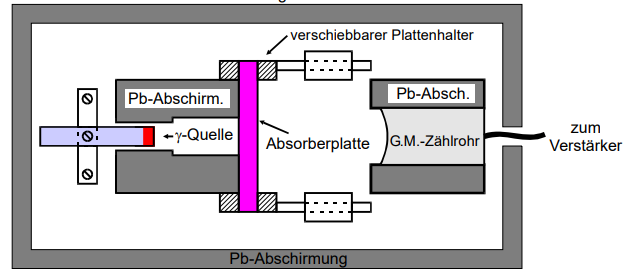
\includegraphics[width=\textwidth]{content/aufbau.png}
        \caption{Aufbau der Messaparatur für die $\gamma$-Absorption\cite[243]{V704}.}
        \label{fig:aufbau}
    \end{figure}

\subsection{Bestimmung der Beta-Absorptionskurven}    
Bei der Messung der $\beta$-Strahlung wird analog zur $\gamma$-Strahlung vorgegangen. Hierbei wird bei einer Absorberdicke von $(482 \pm 1) \symup{\mu m}$ 
und einer Messdauer von $1100$ s angefangen und dann zehn Messungen bis zu einer Dicke von $100 \symup{\mu m}$ durchgeführt.
Als $\beta$-Quelle dient hierbei $\ce{^{99} Tc}$.